\newpage
\chapter{Misiones semejantes}\label{semejantes}
\minitoc

En este apartado, se pretende revisar y comparar las características principales de misiones previas que han abordado retos similares en términos de resolución espacial, cobertura, requisitos espectrales, y diseño de la misión. Finalmente se realiza una tabla comparativa con las características de cada misión que son interesantes para inspirar el presente trabajo.

\newpage

\section{OCO-2 (\textit{Orbiting Carbon Observatory})}

\begin{figure}[h]
    \centering
    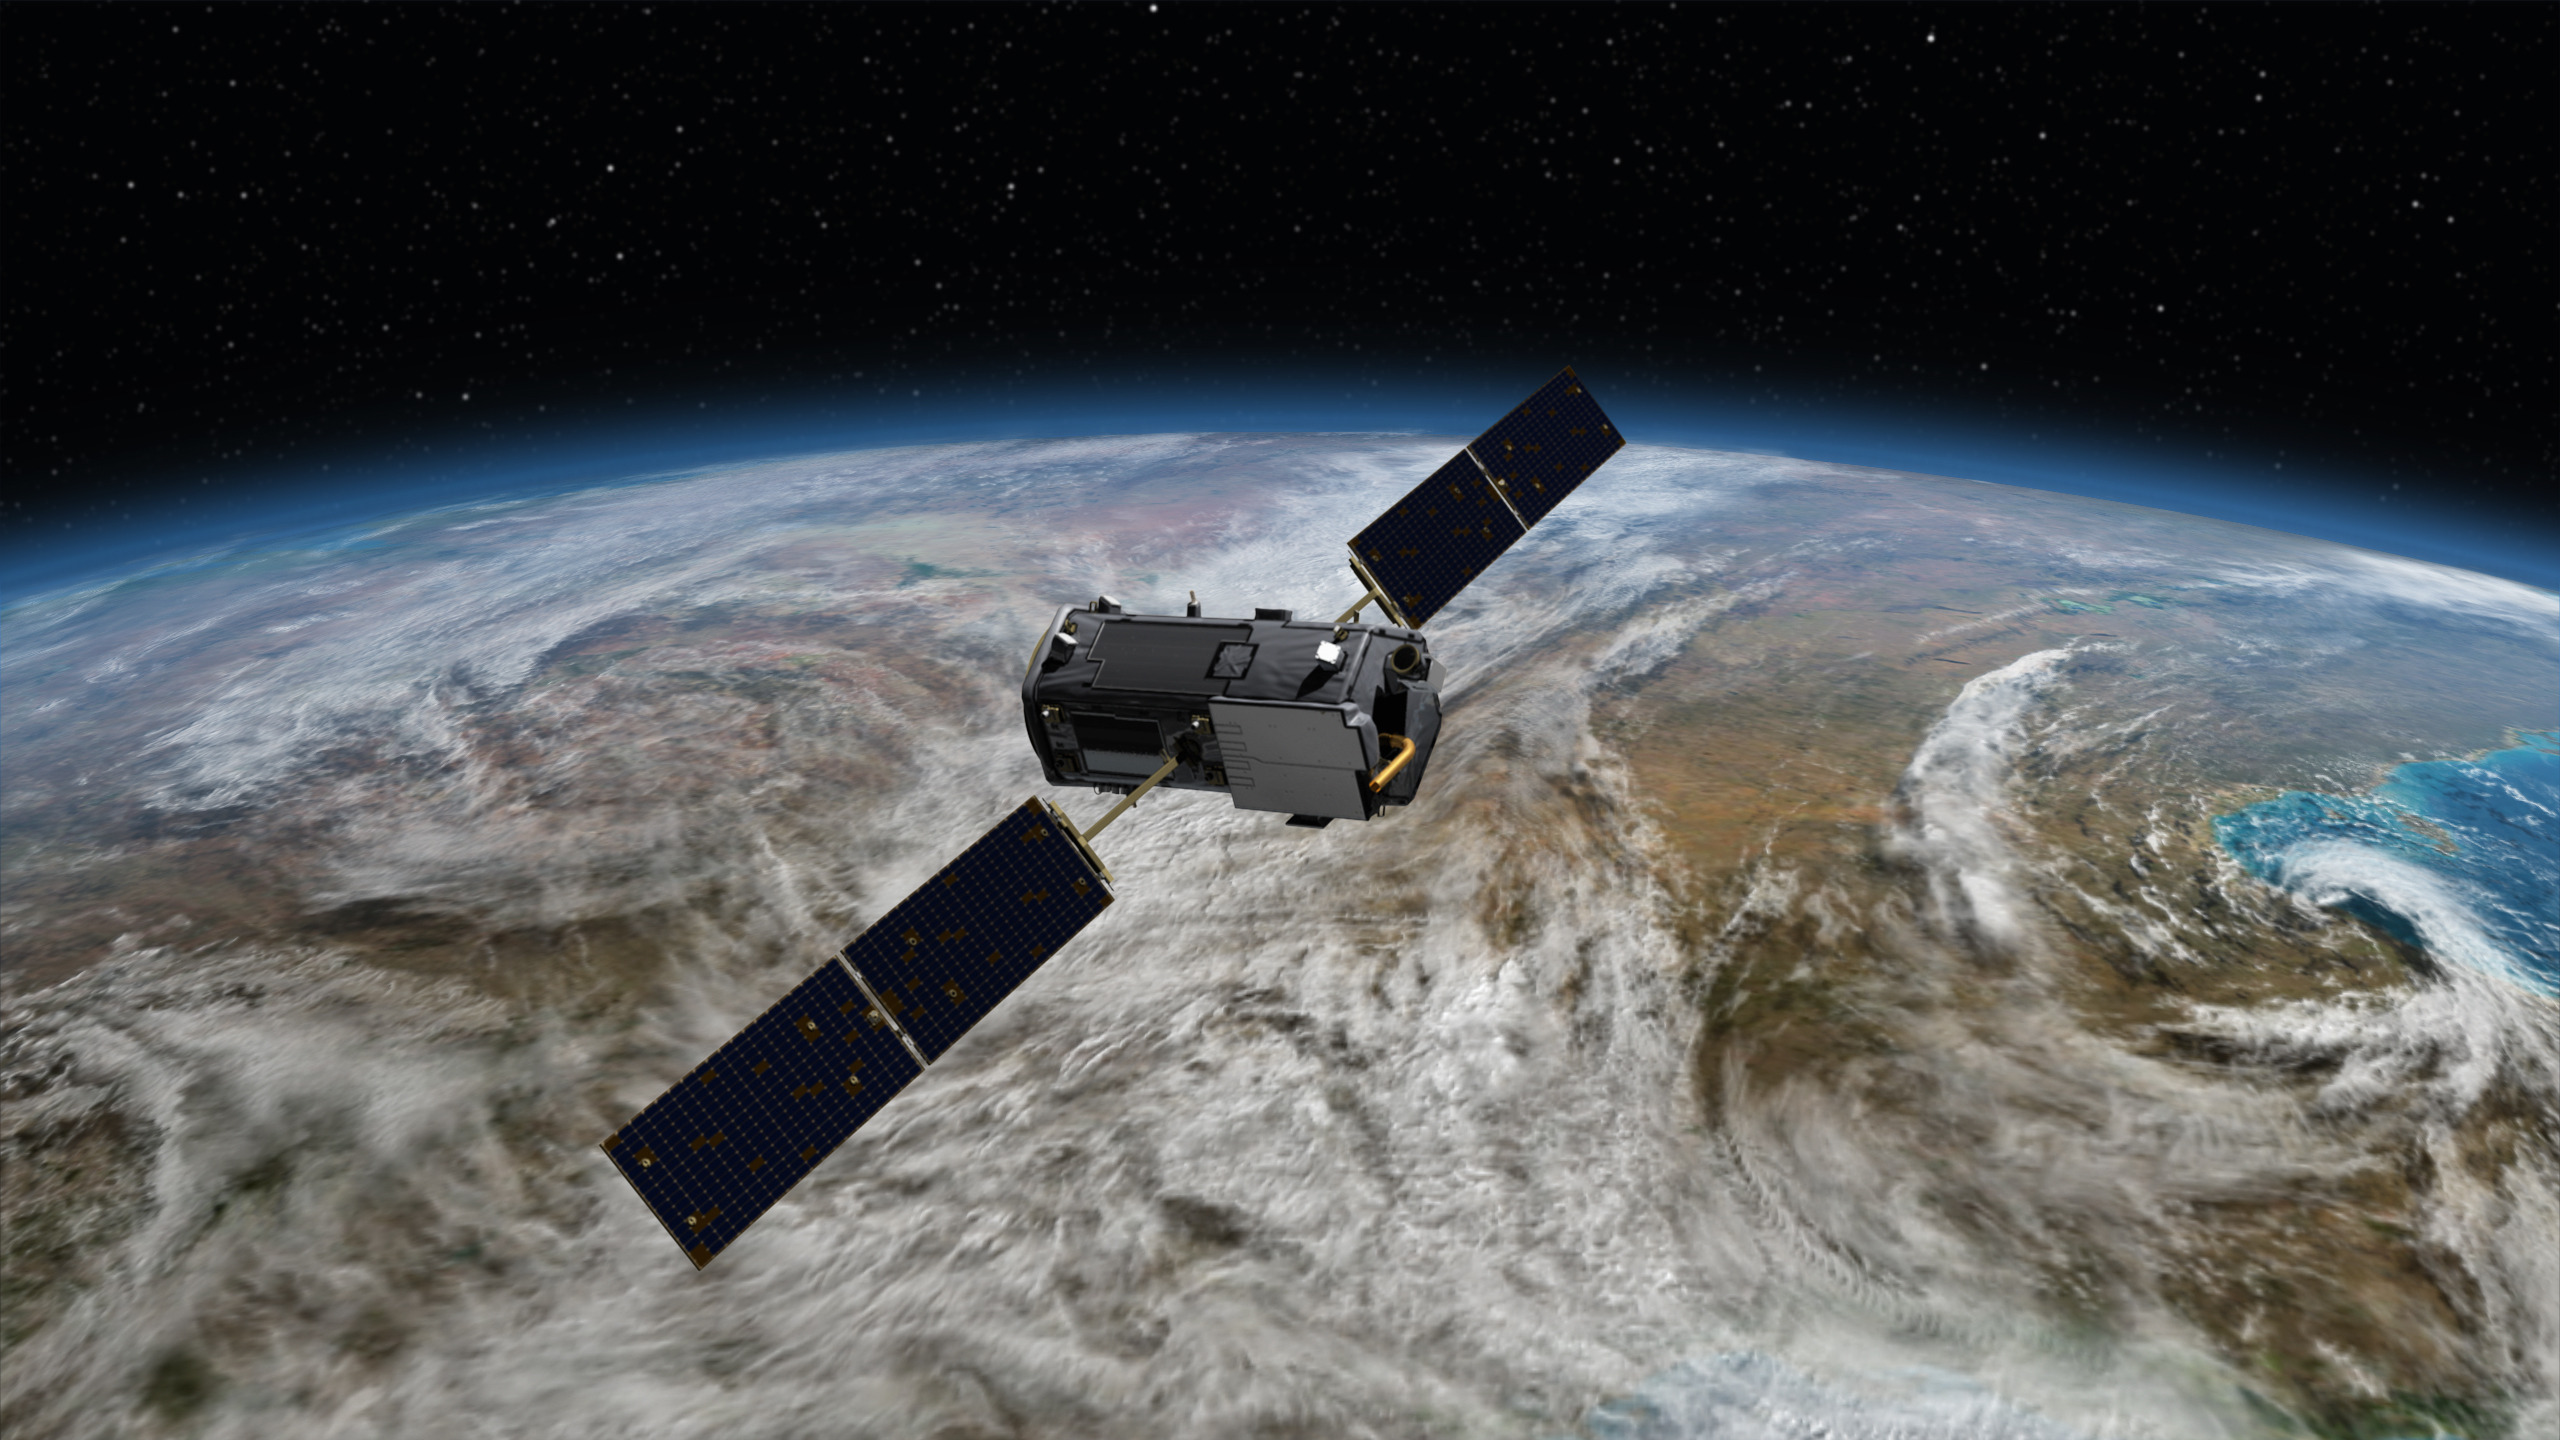
\includegraphics[width=0.9\linewidth]{2.Misiones_Semejantes/OCO2.jpg}
    \caption{Representación artística del \textit{Orbiting Carbon Observatory }(OCO)-2 de la NASA. \\Fuente: \cite{nasa_jpl_oco2_artist_concept_2014}.
}
\end{figure}

OCO-2 representa una de las misiones más significativas dedicadas exclusivamente al monitoreo de CO\textsubscript{2} atmosférico. Lanzado en julio de 2014 por la NASA, este satélite se diseñó para proporcionar mediciones precisas de la concentración de CO\textsubscript{2} a escala global, ofreciendo datos cruciales para la comprensión del ciclo del carbono terrestre.

El satélite emplea tres espectrómetros de rejilla que operan en bandas espectrales del infrarrojo cercano: 0,76 \textmu m (banda O\textsubscript{2} A), 1,61 \textmu m y 2,06 \textmu m (bandas de absorción de CO\textsubscript{2}). Los detectores utilizados son matrices de fotodiodos de silicio HAWAII-1RG fabricados por Teledyne y  mantenidos a -120 °C mediante un sistema criogénico para minimizar el ruido térmico.

El telescopio presenta un diseño Cassegrain con una apertura de 11 cm de diámetro. La resolución espacial alcanza 1,3×2,3 km con un ancho de barrido de 10 km. El satélite orbita a 705 km de altitud en una órbita heliosíncrona con inclinación de 98,2°, proporcionando un período de revisita de 16 días. La masa total del sistema es de 449 kg \cite{eoportal_oco2_2024}.

\section{GOSAT / GOSAT-2 (\textit{Greenhouse Gases Observing Satellite})}

\begin{figure}[H]
    \centering
    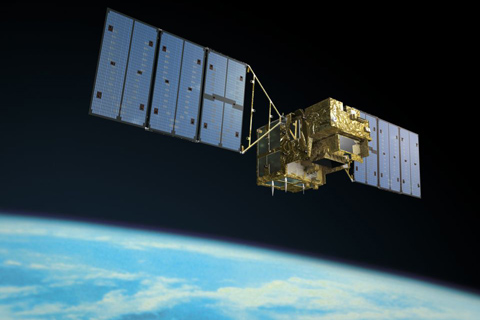
\includegraphics[width=0.8\linewidth]{2.Misiones_Semejantes/gosat_main_001.jpg}
    \caption{Representación artística de GOSAT. \\Fuente: \cite{jaxa_gosat_representation}.
}
\end{figure}

El sistema GOSAT, desarrollado por JAXA, utiliza el espectrómetro de transformada de Fourier TANSO-FTS, GOSAT-1 incorpora las siguientes bandas: Banda 1 (0,758-0,775 \textmu m) centrada en la banda de absorción del oxígeno A, Banda 2 (1,56-1,72 \textmu m) optimizada para la detección de CO\textsubscript{2} y CH\textsubscript{4}, Banda 3 (1,92-2,08 \textmu m) diseñada para CO\textsubscript{2} y H\textsubscript{2}O, y Banda 4 (5,56-14,3 \textmu m) que abarca el infrarrojo térmico para CO\textsubscript{2} y CH\textsubscript{2}. Los detectores empleados incluyen tecnología de silicio (Si) para la banda 1, InGaAs para las bandas 2 y 3, y PC-MCT (\textit{Mercury Cadmium Telluride}) para la banda 4 en el infrarrojo térmico. El telescopio presenta una apertura de 68 mm de diámetro.

La resolución espacial nominal es de 10,5 km en nadir. GOSAT-2, la versión mejorada lanzada en octubre de 2018, opera a 613 km de altitud en órbita heliosíncrona con inclinación de 98,1°, ofreciendo un período de revisita de 6 días. La masa del sistema alcanza aproximadamente 1.700 kg (masa seca), con una masa total inferior a 2.000 kg.

GOSAT-2 incorpora mejoras significativas respecto a su predecesor, incluyendo cinco bandas espectrales (en lugar de cuatro) con rangos optimizados, capacidad para medir monóxido de carbono (CO) adicional al CO\textsubscript{2} y CH\textsubscript{4}, y un mecanismo de apuntamiento inteligente para evitar nubes \cite{jaxa_gosat} \cite{gogoi2023gosat}.

\section{CO2M (\textit{Carbon Dioxide Monitoring Mission})}

\begin{figure}[H]
    \centering
    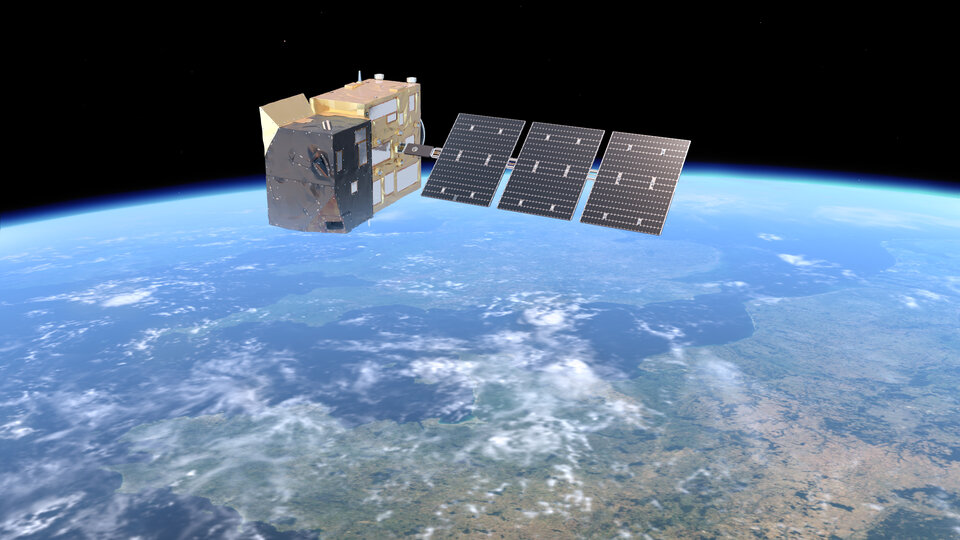
\includegraphics[width=0.8\linewidth]{2.Misiones_Semejantes/Copernicus_Carbon_Dioxide_Monitoring_mission_article-2326145821.jpg}
    \caption{CO2M, de la Agencia Espacial Europea. \\Fuente: \cite{CO2M}.
}
\end{figure}

CO2M representa una iniciativa pionera de la Agencia Espacial Europea (ESA) dentro del programa Copernicus, diseñada específicamente para monitorizar las emisiones antropogénicas de CO\textsubscript{2} a escala global. Programada para lanzarse a partir de 2025, esta misión constará de una constelación de tres satélites (CO2M-A, CO2M-B y CO2M-C) que trabajarán en conjunto para proporcionar una cobertura temporal sin precedentes.


El instrumento principal, denominado CO2I (Integrated CO\textsubscript{2} and NO\textsubscript{2} Imaging Spectrometer), es un espectrómetro de alta precisión que opera en múltiples bandas espectrales: 405-490 nm (visible), 747-773 nm (infrarrojo cercano) y dos rangos de infrarrojo de onda corta (1,59-1,67 \textmu m y 1,98-2,08 \textmu m). Los detectores utilizados son de tecnología MCT (\textit{Mercury Cadmium Telluride}). Con una resolución espacial de 4 km\textsuperscript{2}, el sistema está optimizado para identificar fuentes puntuales como centrales eléctricas y complejos industriales.


Una característica distintiva de CO2M es su sistema integrado de corrección atmosférica, que combina el instrumento CLIM (imagen de nubes en tres bandas) y el MAP (polarímetro multiangular) para filtrar datos afectados por cubierta nubosa. La constelación completa logrará una revisita global cada 3,5 días, útil para el monitoreo efectivo de áreas urbanas dinámicas, con una masa aproximada de 900 kg por satélite \cite{CO2M} \cite{CO2M_progress}.

\section{TanSat (\textit{Chinese Carbon Dioxide Observation Satellite})}

\begin{figure}[H]
    \centering
    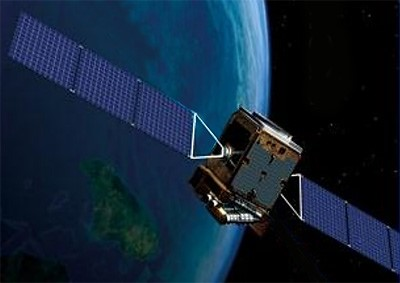
\includegraphics[width=0.8\linewidth]{2.Misiones_Semejantes/tansat.jpg}
    \caption{TanSat. \\Fuente: \cite{tansat}.
}
\end{figure}

TanSat, lanzado en diciembre de 2016 por la Academia China de Ciencias, se convirtió en el primer satélite chino dedicado específicamente a la monitorización de CO\textsubscript{2}. Su objetivo principal es medir la concentración de dióxido de carbono en la atmósfera con alta precisión y contribuir a la comprensión del ciclo global del carbono.

TanSat incorpora dos instrumentos principales: un espectrómetro de CO\textsubscript{2} de alta resolución (CarbonSpec) que opera en las bandas de 0,76 \textmu m (banda de oxígeno A), 1,61 \textmu m y 2,06 \textmu m (bandas de CO\textsubscript{2}), y un polarímetro de nube y aerosol (CAPI) que observa en siete bandas espectrales desde el ultravioleta hasta el infrarrojo cercano. Los detectores utilizados son matrices de fotodiodos de InGaAs (Indio, Galio, Arsénico) para las bandas de CO\textsubscript{2}.

El telescopio utiliza un diseño óptico tipo Offner que proporciona una resolución espacial de 2 km × 2 km con un ancho de barrido de 20 km. Este satélite orbita a una altitud de aproximadamente 700 km en una órbita heliosíncrona con inclinación de 98,2°, similar a la de OCO-2. Su masa total es de aproximadamente 620 kg \cite{eoportal_tansat}.

\section{MicroCarb (\textit{Microsatellite for Carbon Observation})}

\begin{figure}[H]
    \centering
    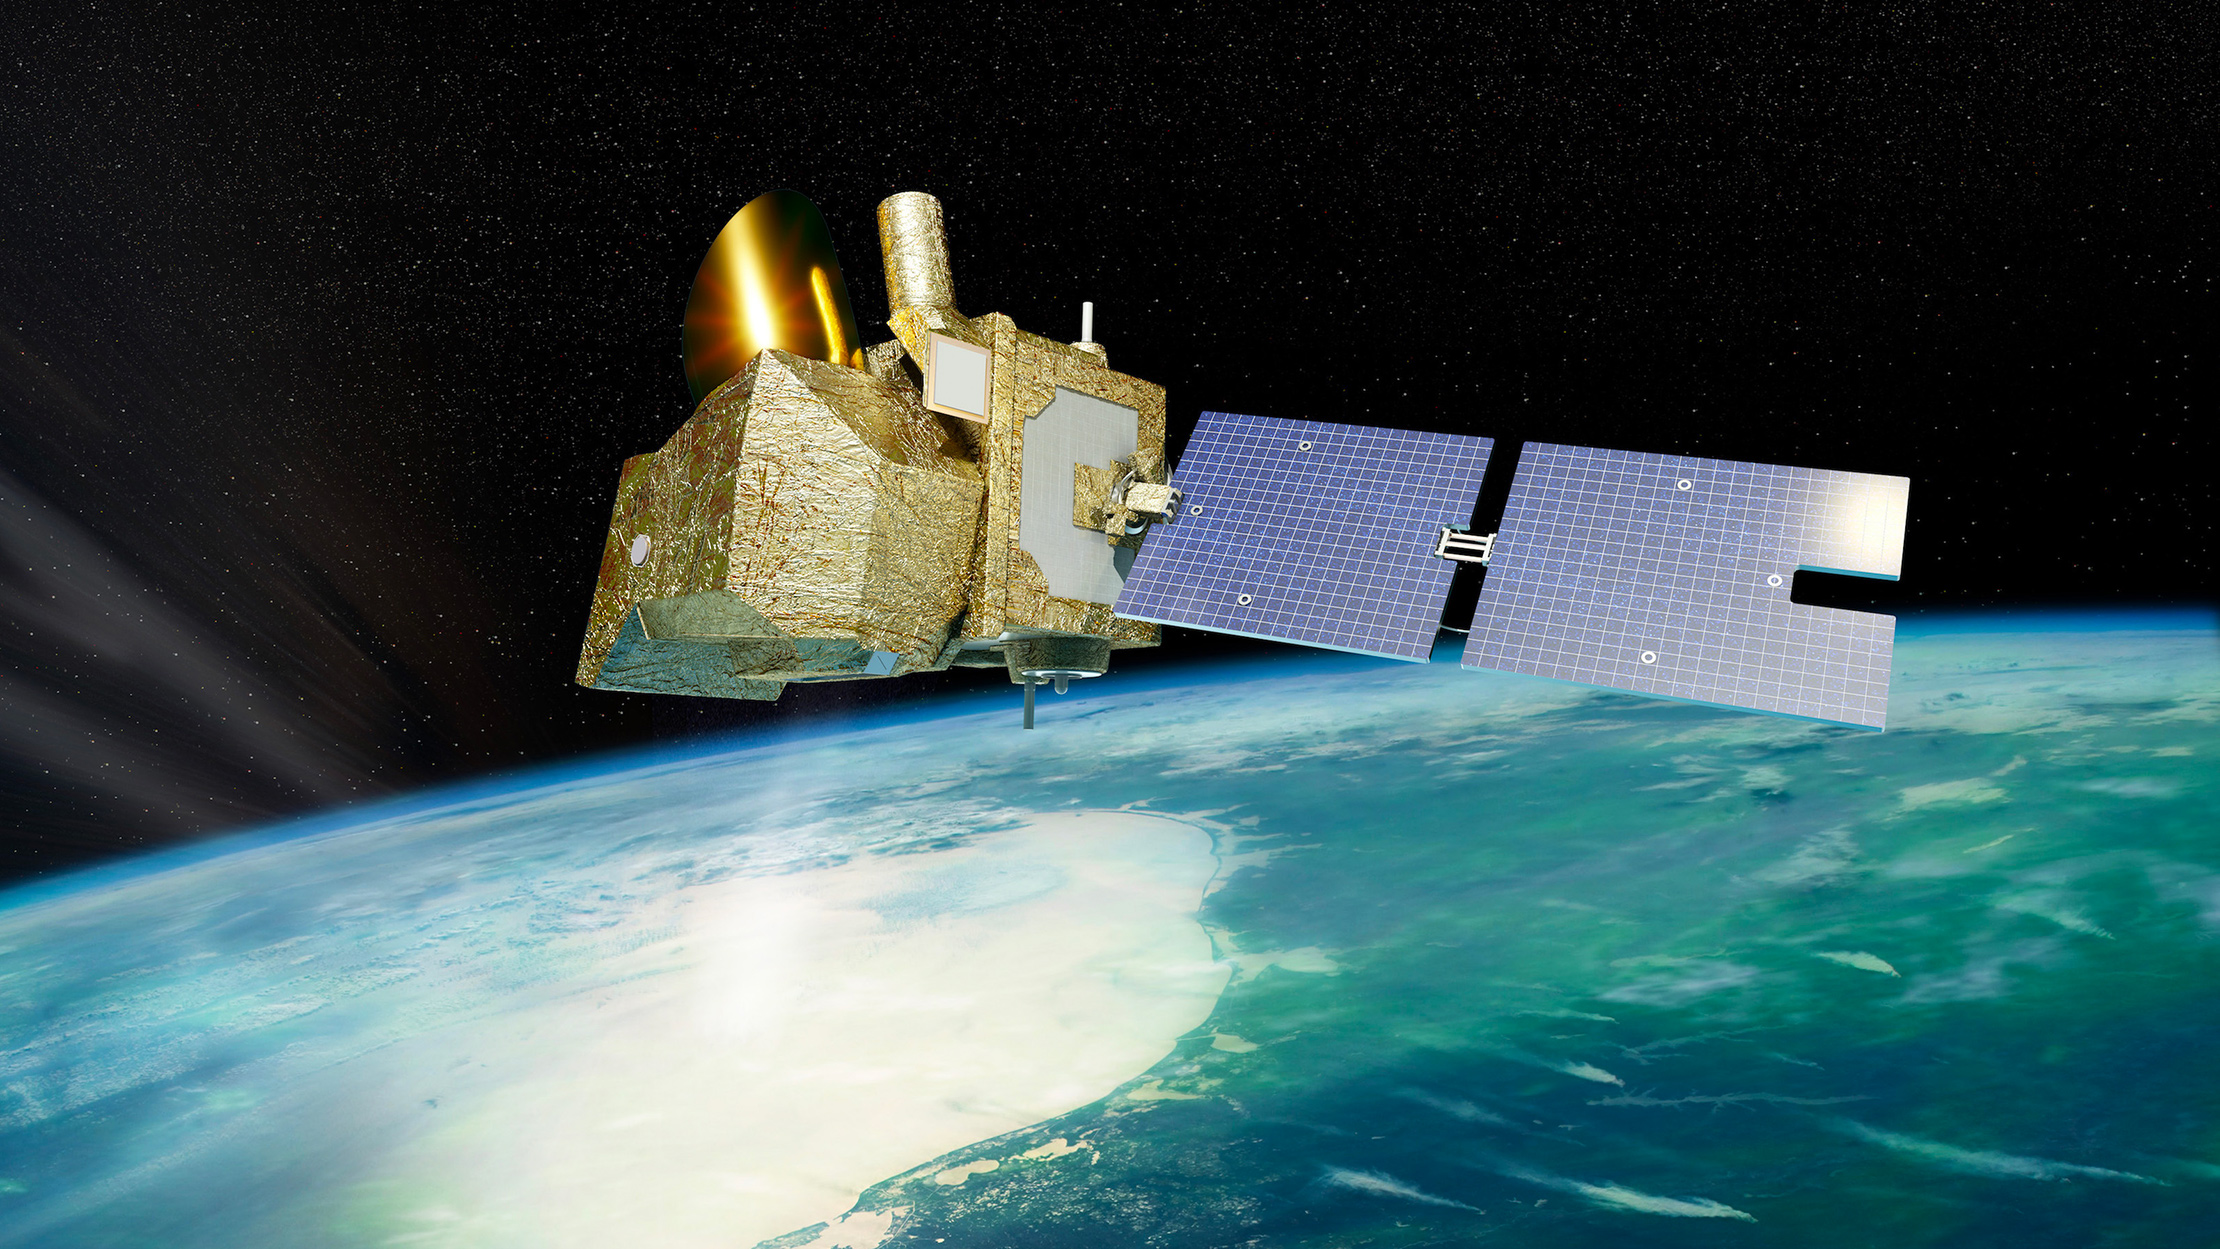
\includegraphics[width=0.8\linewidth]{2.Misiones_Semejantes/Microcarb_Airbus_Cnes_OliverSattler-1386146461.jpg}
    \caption{Imagen artistica de Microcarb. \\Fuente: \cite{futura_microcarb}
}
\end{figure}

MicroCarb es una misión desarrollada por la agencia espacial francesa CNES, con lanzamiento previsto en 2025. Representa un enfoque innovador al utilizar una plataforma de microsatélite para realizar mediciones precisas de CO$_\textsubscript{2}$ atmosférico, demostrando que misiones efectivas pueden implementarse con presupuestos y masas reducidas.

El instrumento principal de MicroCarb es un espectrómetro de rejilla compacto que opera en cuatro bandas espectrales: 0.76 \textmu m (O\textsubscript{2}), 1.27 \textmu m (O\textsubscript{2}), 1.6 \textmu m (CO\textsubscript{2}) y 2.01 \textmu m (CO\textsubscript{2}). Esta configuración permite mediciones precisas de concentración de CO\textsubscript{2} con una resolución espacial aproximada de 4.5 km × 9 km. Permite además alcanzar una resolución máxima de 2 km × 2 km en modo de escaneo urbano. 

MicroCarb operará en una órbita heliosíncrona a aproximadamente 650 km de altitud con un período de revisita de 25 días. Lo que destaca de esta misión es su masa total de solo 180 kg, significativamente menor que otras misiones similares, demostrando los avances en la miniaturización de tecnologías espaciales \cite{eoportal_microcarb}.

\section{GHGSat}

\begin{figure}[H]
    \centering
    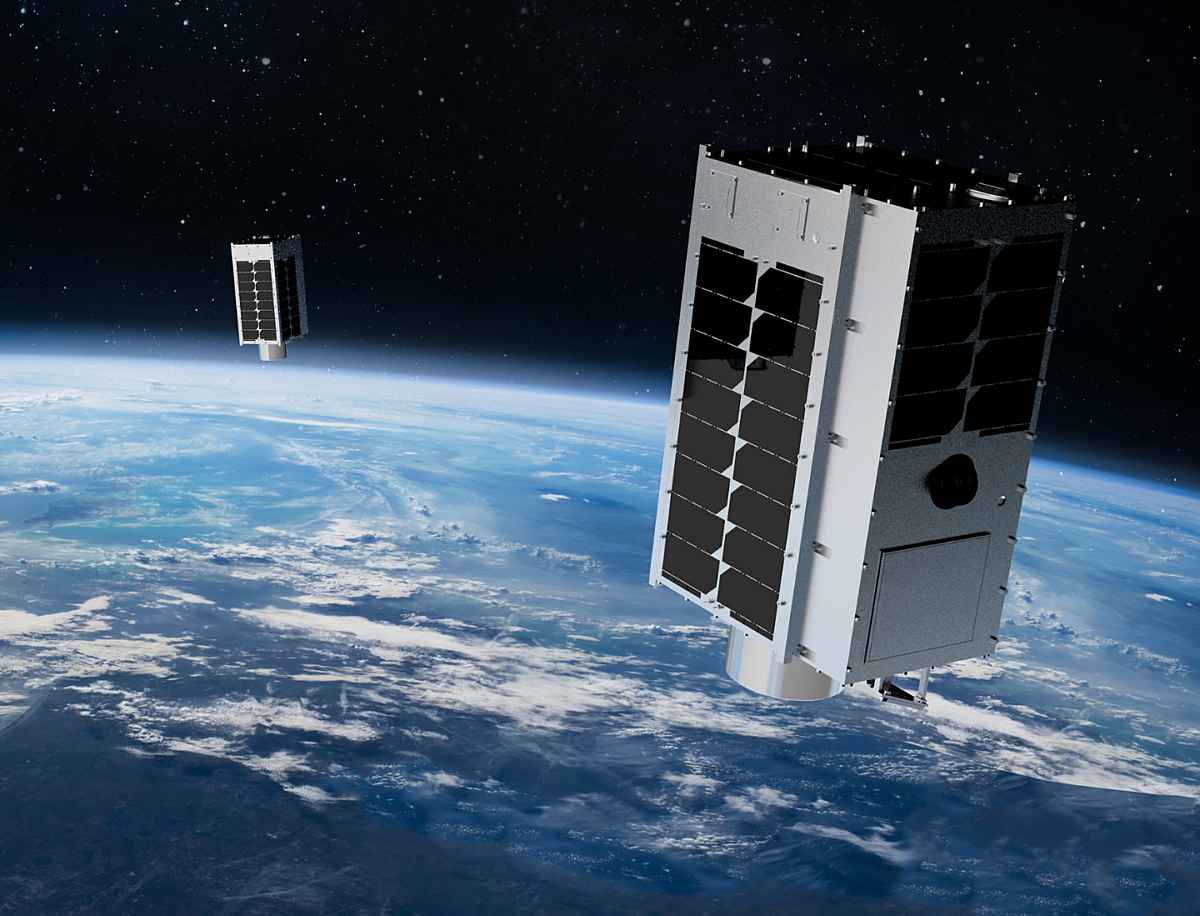
\includegraphics[width=0.8\linewidth]{2.Misiones_Semejantes/GHGSat_Constellation-of-Six-Satellites_1440x1100-2772752015.png}
    \caption{Constelacion GHGSat. \\Fuente: \cite{gosat_gw}
}
\end{figure}

La constelación GHGSat representa un enfoque comercial al monitoreo de gases de efecto invernadero. Esta constelación se dedica a la detección de emisiones de metano y CO$_\textsubscript{2}$ a nivel de instalaciones individuales, ofreciendo una resolución espacial sin precedentes para aplicaciones específicas de monitorización de fuentes puntuales.


Cada satélite GHGSat está equipado con un espectrómetro de imagen compacto denominado WAF-P (Wide-Angle Fabry-Perot) que opera en bandas del infrarrojo cercano específicas para la detección de metano y CO\textsubscript{2}. Los detectores utilizados son de tecnología InGaAs, optimizados para la detección en el rango espectral de 1600-1700 nm. El telescopio emplea un diseño reflectivo con una apertura de aproximadamente 5 cm.


La tecnología patentada permite una resolución espacial de aproximadamente 25 metros, capacitando la identificación precisa de fuentes de emisión. Los satélites GHGSat operan en órbitas heliosíncronas a altitudes entre 500-550 km con una inclinación de 97,5°. Cada unidad tiene una masa de aproximadamente 15-20 kg, ejemplificando el potencial de los nanosatélites para aplicaciones de observación terrestre especializadas \cite{wmo_ghgsat_spectrometer}.






\section{Hallazgos clave}
Primeramente se presenta una tabla comparativa con el fin de resumir las principales características de las misiones analizadas:



\begin{landscape}
\begin{table}[p]
\centering
\caption{Comparativa de misiones de observación de CO\textsubscript{2}.}
\small
\begin{tabular}{lcccccc}
\toprule
\textbf{Parámetro} & \textbf{OCO-2} & \textbf{GOSAT2} & \textbf{CO2M} & \textbf{TanSat} & \textbf{MicroCarb} & \textbf{GHGSat} \\
\midrule
Detector & Fotodiodos Si  & InSb/MCT & MCT & InGaAs & MCT & InGaAs \\
Diámetro pupila (cm) & 11 & 10 & 15 & 12 & 8 & 5 \\
GSD (km) & 1.3$\times$2.3 & 10 & 2 & 2 & 4.5 & 0.025 \\
Swath (km) & 10 & 10 & 250 & 20 & 250 & 12 \\
Altura orbital (km) & 705 & 666 & 735 & 700 & 650 & 500 \\
Tipo órbita & SSO 98.2° & SSO 98.1° & SSO 97.7° & SSO 97.4° & SSO 98.0° & SSO 97.6° \\
Constelación & No & No & Sí (3) & No & No & Sí (10+) \\
Tipo telescopio & Cassegrain & FTS & Cassegrain & Offner & Off-axis & Reflective \\
Duración (años) & 2 (+10) & 5 & 7.5 & 5 & 3 & 5 \\
Revisita (días) & 16 & 3 & 3.5 & 16 & 25 & 5 \\
Masa (kg) & 450 & 2900 & 900 & 600 & 180 & 15 \\
Paneles solares (m$^2$) & 8 & 24 & 12 & 10 & 4 & 1.8 \\
Cobertura & Global & Global & Global & Global & Global & Puntual \\
\bottomrule
\end{tabular}

\end{table}
\end{landscape}

Del análisis comparativo de las estas misiones se pueden extraer los siguientes hallazgos clave, que serán útiles para inspirar la misión encomendada:

\begin{itemize}
    \item Las misiones analizadas muestran diferentes aproximaciones al monitoreo de CO\textsubscript{2}, desde satélites individuales de gran tamaño (GOSAT-2) hasta constelaciones de microsatélites (GHGSat), pasando por soluciones intermedias como MicroCarb.
    \item Se utilizan diferentes tecnologías de detección según los requerimientos específicos de cada misión, desde fotodiodos de silicio (OCO-2) hasta detectores de InGaAs (TanSat, GHGSat) y MCT (GOSAT-2, CO2M)
    \item Las constelaciones como CO2M y GHGSat logran períodos de revisita significativamente menores (3,5 y 5 días respectivamente) que los satélites individuales, mejorando la capacidad de monitoreo temporal.
    \item La selección universal de órbitas heliosíncronas en todas las misiones analizadas demuestra su importancia crítica para la observación terrestre. Esta configuración orbital garantiza condiciones de iluminación consistentes al pasar sobre cualquier punto de la superficie terrestre a la misma hora solar local, lo que resulta fundamental para la comparabilidad temporal de los datos espectrales. Adicionalmente, la órbita heliosíncrona facilita la cobertura global sistemática con períodos de revisita predecibles, optimizando tanto la adquisición de datos como la planificación de misiones de monitoreo ambiental.

\end{itemize}